\documentclass{ctexart}
\usepackage{tikz}
\usepackage{amsmath}
\usepackage{mathtools}
\usepackage{listings}
\usepackage{xcolor}
\usepackage{float}
\usepackage{graphicx}
\usepackage{geometry}

\geometry{a4paper,left=3cm,right=3cm}
\title{计算物理学作业}
\author{艾鑫}

\lstset{flexiblecolumns}
\lstset{
  basicstyle=\sffamily,
  keywordstyle=\bfseries\color{blue!70},
  frame=shadowbox,
  commentstyle=\color{red!50!green!50!blue!50},% \rmfamily\itshape
  stringstyle=\ttfamily,
  rulesepcolor=\color{red!20!green!20!blue!20}
}

\newcounter{mycnt}
\setcounter{mycnt}{0}
\newenvironment{problem}[1][1.1]{\noindent \stepcounter{mycnt}\themycnt.(#1)}{

}

\newenvironment{answer}{\textbf{解}:}{
\vspace{0.5cm}
}

\newcommand\diff{\,\mathrm{d}}

\begin{document}
\maketitle

\begin{problem}[3.10]
用4点高斯求积公式编程计算积分
\begin{equation}
  I = \int_{1.4}^{2.0} \int_{1.0}^{1.5} \ln (x+2y) \diff x \diff y
\end{equation}
\end{problem}

\begin{answer}
  将积分区间$R = \{(x,y)|1.4 \leq x \leq 2.0, \, 1.0 \leq y \leq 1.5\}$变换到$R' = \{(u,v)|-1 \leq u \leq -1, \, -1 \leq v \leq 1\}$, 即有
  \begin{equation}
    \left\{
      \begin{lgathered}
        x = \frac{1}{2}(b_2 + a_2) + \frac{1}{2} (b_2 - a_2)u \\
        y = \frac{1}{2}(b_1 + a_1) + \frac{1}{2} (b_1 - a_1)v
      \end{lgathered}
    \right.
  \end{equation}
因此有
\begin{equation}
  I = 0.0755 \int_{-1}^{1} \int_{-1}^{1} \ln (0.3 u + 0.5 v + 4.2) \diff u \diff v
\end{equation}
使用$n=3$的4点高斯求积公式, 利用MATLAB求解得
\begin{equation}
  \begin{split}
  I &= \int_{1.4}^{2.0} \int_{1.0}^{1.5} \ln (x+2y) \diff x \diff y \\
    &= 0.429554527717559
  \end{split}
\end{equation}

MATLAB代码如下:
\begin{lstlisting}[language=Octave]
% 第一题 用四点高斯求积公式求二重积分

node = [0.3399810, 0.8611363];
coef = [0.6521452, 0.3478548];

u = [-node(2),-node(1),node(1),node(2)];
v = u;
A = [coef(2),coef(1),coef(1),coef(2)];

s = 0;

for i = 1:4
    for j = 1:4
	s = s + A(i)*A(j)*log(0.3*u(i) + 0.5*v(j) + 4.2);
    end
end

I = 0.075 * s;

format long
disp(I)
\end{lstlisting}

\end{answer}

\begin{problem}[4.7]
  应用龙格-库塔法求初值问题
  \begin{equation}
    \left\{
    \begin{lgathered}
      y'' + 2ty' + t^2 y = e^t, \quad 0 \leq t \leq 1 \\
      y(0) = 1, y'(0) = -1
    \end{lgathered}
    \right.
  \end{equation}
的数值解,取步长$h = 0.1$.
\end{problem}

\begin{answer}
  令$y_1 = y, y_2 = y'$, 问题则转化为
  \begin{equation}
    \left\{
      \begin{lgathered}
        y_1' = y_2 \\
        y_2' = e^t - 2ty_2 - t^2y_1, \quad 0\leq t \leq 1 \\
        y_1(0) = 1, \, y_2(0) = -1
      \end{lgathered}
    \right.
  \end{equation}

应用龙格-库塔法求得解如下图所示:
\begin{figure}[H]
  \centering
  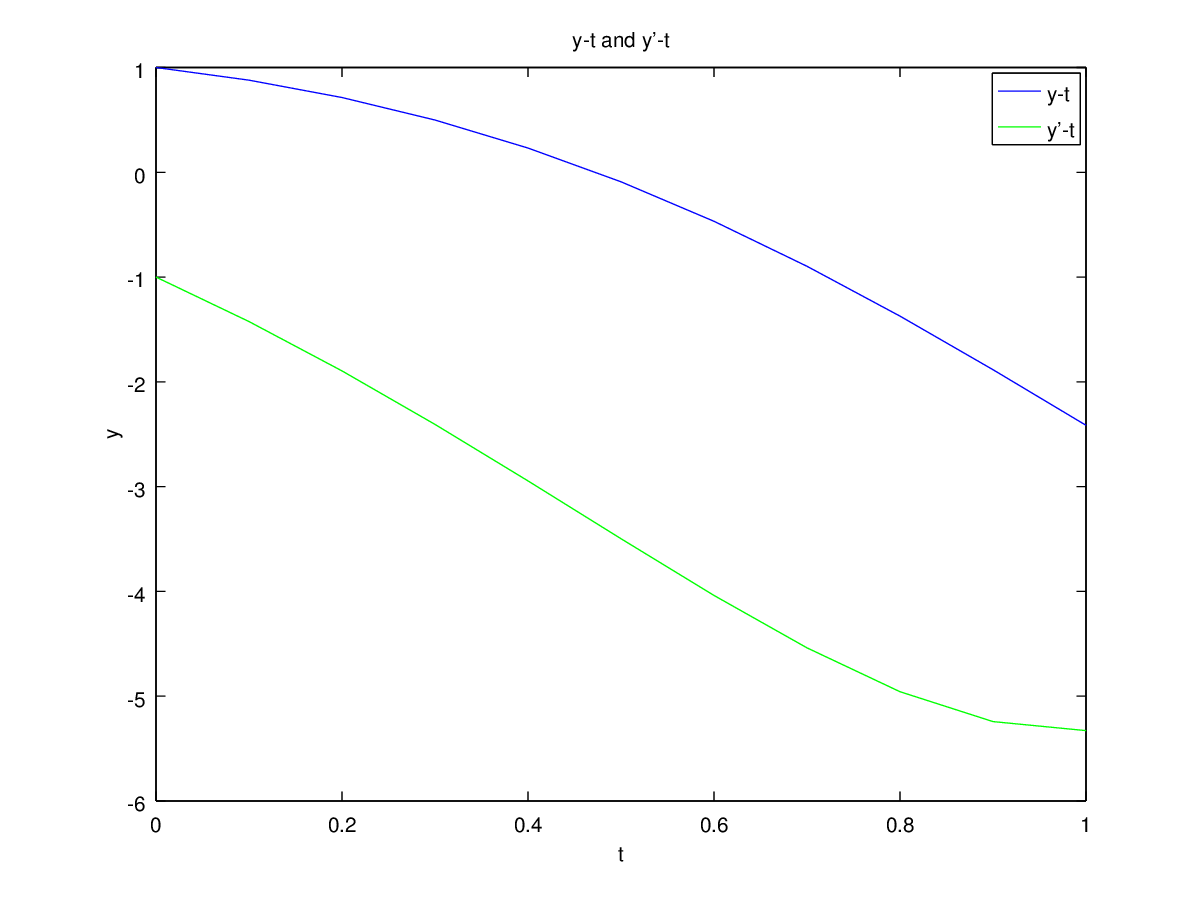
\includegraphics[width=7cm]{code/fig1.png}
  \caption{龙格-库塔法求解结果}
\end{figure}

MATLAB代码如下:
\begin{lstlisting}[language=Octave]
% 第二题 应用龙格-库塔法求初值问题
% 设置初始值
t0 = 0;
h = 0.1;

y1_0 = 1;
y2_0 = -1;

function K = fun(t, y)
  f1 = y(2);
  %f2 = exp(t) - 2*t*y(2) - t^2*y(1);
  f2 = exp(2*t)*sin(t) - 2*y(1) + 2*y(2);
  K = [f1,f2];
endfunction

t = 0:h:1;
n = size(t,2);
Y = zeros(n,2);
Y(1,1) = y1_0;
Y(1,2) = y2_0;

for i = 1:n-1
  K1 = fun(t(i), Y(i,:));
  K2 = fun(t(i) + h/2, Y(i,:) + (h/2)*K1);
  K3 = fun(t(i) + h/2, Y(i,:) + (h/2)*K2);
  K4 = fun(t(i) + h, Y(i,:) + h*K3);
  Y(i+1,:) = Y(i,:) + (K1 + 2*K2 + 2*K3 + K4) * (h/6);
end
% 画图
plot(t,Y(:,1)','b',t,Y(:,2)','g')
xlabel('t')
ylabel('y')
legend('y-t',"y'-t")
title("y-t and y'-t")
\end{lstlisting}
\end{answer}

\begin{problem}[8.4]
  试采用有限差分法编程求解单位圆域中泊松方程在网格节点处的值
  \begin{equation}
    \left\{
      \begin{lgathered}
        \nabla^2u = -50r^2 \sin (2\phi) \\
        u(1, \phi) = 0
      \end{lgathered}
    \right.
  \end{equation}
  其中$u(1,\phi)=0$表示半径为1的单位圆边界上$u$值为$1$. 取$h = 0.1, \omega = 1.25, \varepsilon = 10^{-5}, M = 16$, 并与解析解$u = \frac{25}{6}r^2(1-r^2) \sin(2\phi)$作比较.
\end{problem}

\begin{answer}
在极坐标下泊松方程形式为
\begin{equation}
  \nabla^2u = \frac{\partial^2u}{\partial r^2} + \frac{1}{r}\frac{\partial u}{\partial r} + \frac{1}{r^2}\frac{\partial^2u}{\partial \varphi^2} = -50r^2 \sin (2\phi)
\end{equation}

用一组等角线和等距离同心圆分割区域, 将半径$N-1$等分, 圆周$M-1$等分, 即有
\begin{equation}
  \left\{
    \begin{lgathered}
      \Delta r = h = \frac{r_0}{N-1} \\
      \Delta \varphi = \frac{2\pi}{M-1}
    \end{lgathered}
  \right.
\end{equation}

用误差为$\mathrm{O}(\Delta r^2)$和$\mathrm{O}(\Delta \varphi^2)$的中心差商代替上式中的微商, 可以得到泊松方程的差分格式为
\begin{equation}\label{possion}
  \alpha_0(u_{i,j-1} + u_{i,j+1}) + \alpha_1u_{i-1,j} + \alpha_2u_{i+1,j} - 2(1+\alpha_0)u_{ij} = h^2 f(r_i,\varphi_j)
\end{equation}
其中, $\alpha_0 = [\Delta\varphi(i-1)]^{-2}, \alpha_1 = 1 - (2i-2)^{-1}, \alpha_2 = 1 + (2i-2)^{-1}$.
\end{answer}

周期性条件有
\begin{equation}
  u(r,\varphi)  u(r, \varphi + 2\pi)
\end{equation}
即满足$u_{i1} = u_{iM}, u_{i2} = u_{i,M+1}$.

方程\eqref{possion}不适合于圆心($i=1$). 利用直角坐标系下的五点差分格式,有
\begin{equation}
  \nabla^2u_0 \approx \frac{1}{h^2}(u_1 + u_2 + u_3 + u_4 - 4u_0)
\end{equation}
在一般情况下, 可将上式写为
\begin{equation}
  \nabla^2 u_0 = \frac{4}{h^2} (\bar{u} - u_0)
\end{equation}
其中$\bar{u}$是半径为$h$的圆周上各结点的平均值, 即
\begin{equation}
  \bar{u} = \frac{1}{M-1} \sum_{j = 2}^{M} u_{2j}.
\end{equation}

下面对\eqref{possion}进行简化, 可得
\begin{equation}
  u_{ij} = \frac{\alpha_0(u_{i,j-1} + u_{i,j+1}) + \alpha_1u_{i-1,j} + \alpha_2u_{i+1,j} - h^2f(r_i, \varphi_j)}{2+2\alpha_0}
\end{equation}
引入超松弛因子, 进行超松弛迭代
\begin{equation}
  u_{ij}^{k+1} = \omega \times \frac{\alpha_0(u_{i,j-1}^{k+1} + u_{i,j+1}^{k+1}) + \alpha_1u_{i-1,j}^{k+1} + \alpha_2u_{i+1,j}^{k+1} - h^2f(r_i, \varphi_j)}{2+2\alpha_0} + (1-\omega)\times u_{ij}^k
\end{equation}
通过编程求解得结果如下, 与解析解的最大误差为0.025092.

MATLAB代码如下:
\begin{lstlisting}[language=Octave]
% 第三题 用有限差分法求解单位园域中的泊松方程
% 设置初始值
omega = 1.25;
epsilon = 10^(-7);
r0 = 1.0;
h = 0.1;
deltaR = h;
global N = r0/h+1;
global M = 16;
deltaPhi = 2*pi/(M-1);

R = 0:deltaR:r0;
Phi = 0:deltaPhi:2*pi;
U = zeros(N,M);
% 定义下标i的转换函数, 依据周期性条件
function newi = subi(i)
  global N;
  if i==0
    newi = N-1;
  elseif i == N+1
    newi = 2;
  elseif i == N
    newi = 1;
  else
    newi = i;
  end
endfunction
% 定义下标j的转换函数, 依据周期性条件
function newj = subj(j)
  global M;
  if j==0
    newj = M-1;
  elseif j == M+1
    newj = 2;
  elseif j == M
    newj = 1;
  else
    newj = j;
  end
endfunction

function y = fun(r, phi)
  y = -50 * r^2 * sin(2*phi);
endfunction
% 进行迭代
do
  maxDiffU = 0;
  for i = (N-1):-1:1 
    if i==1 % 判断是否为圆心
      oldU = U(1,1);
      meanU = mean(U(2,1:(M-1)));
      U0 = omega*(meanU - h^2/4*fun(R(i),Phi(j))) + (1-omega)*oldU;
      U(1,:) = U0;
      diffU = abs(U(1,1)-oldU);
      if diffU > maxDiffU
	maxDiffU = diffU;
      end
    else 
      for j = 1:M-1
	oldU = U(i,j);
	alpha_0 = (deltaPhi*(i-1))^(-2);
	alpha_1 = 1 - (2*i-2)^(-1);
	alpha_2 = 1 + (2*i-2)^(-1);
	fenmu = 2*(1+alpha_0);

	temp1 = alpha_0 * ( U(subi(i),subj(j-1)) + \
			    U(subi(i),subj(j+1)) );
	temp2 = alpha_1 * U(subi(i-1),subj(j));
	temp3 = alpha_2 * U(subi(i+1),subj(j));
	U(i,j) = omega*(temp1 + temp2 + temp3 - \
			h^2*fun(R(i),Phi(j)) )/fenmu + (1-omega)*U(i,j);
	diffU = abs(U(i,j) - oldU);
	if diffU > maxDiffU
	  maxDiffU = diffU;
	end
      end
    U(i,M) = U(i,1);
    end
  end
until maxDiffU < epsilon
% 计算解析解
realU = zeros(size(U));
for i = 1:N
  for j = 1:M
    realU(i,j) = 25/6*(R(i))^2*(1-(R(i))^2)*sin(2*Phi(j));
  end
end
% 输出结果
disp(max(max(abs(U-realU))))
save -ascii U.dat U
save -ascii realU.dat realU
\end{lstlisting}
\begin{problem}[11.1]
  编程计算例11.1中点3的电势和1,2两点的电量(见图11.9).
\end{problem}

\begin{answer}
测试回答
\end{answer}

\begin{problem}[12.9]
  采用蒙特卡罗方法编程求解一下方程.
  \begin{enumerate}
  \item[(1)] $e^{-x^3}-\tan x + 800 = 0 \,(0 < x < \pi / 2)$;
  \item[(2)] $x + 5e^{-x} - 5 = 0 \, (0 < x < 10)$.
  \end{enumerate}
\end{problem}

\begin{answer}
测试回答
\end{answer}

\end{document}